% Appendices file. here, cover all topics related to thesis.


% PERFORMANCE METRICS ==========================================================
\section{Performance Metrics}
\label{appendix_metrics}
The concept of verifying accuracy in a statistical estimate is covered in [xx source], and some of this information is covered briefly below. In the field of image recognition, one particularly interesting metric is "Intersection over Union", also referred to as IOU or Jaccard Index. From this metric, precision and recall may then be calculated. Precision and recall are fundamental in obtaining more abstracted metrics such as Average Precision and mean Average Precision (mAP), which are how different networks are compared. The following information is primarily taken from the well-known PASCAL VOC (visual objects classes) Challenge \cite{everingham_pascal_2010} and "An Introduction to Information Retrieval" by \cite{manning_introduction_2008}.

\subsection{Defining a Result}
The first step in measuring performance is categorizing what a result may be. With a visual task such as object classification, there are 4 possible outcomes, as shown xbelow. In general, there may be a True Positive, False Positive, True Negative, or False Negative. In practice, True Negatives are not used, and the remaining three are used to varying degrees. Each is better clarified as such:
\begin{itemize} \itemsep=-.5em
	\item True Positive: Correctly detecting a true object
	\item False Positive: Incorrectly detecting something that isn't there
	\item False Negative: Incorrectly ignoring a true object
	\item True Negative: Correctly ignoring something that isn't there
\end{itemize}

\begin{figure}[h] % h = "approx here", {h,t,b}
	\centering
	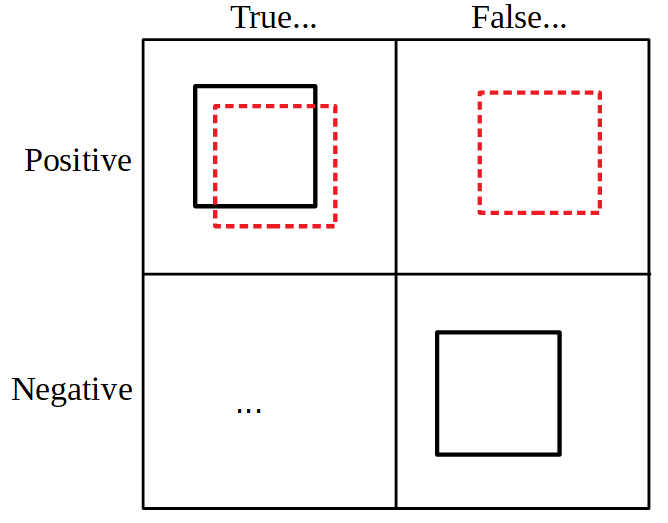
\includegraphics[width=.4\textwidth]{../media/tp_help.png}
	\caption{A visual representation of various outcomes, ground truths as solid black boxes and detections as dotted red boxes. True positives (TP) are a correct detection, FP's are a detection of no actual object, and FN's are a lack of detection of an actual object.}
	\label{tp_help} %label goes last
\end{figure}

To actually classify a result in one of these categories, computer vision depends on using the overlap of a given bounding box estimate with a bounding box ground truth. If the overlap is above some threshold, the estimate is said to be a true positive. In some metrics, two estimates overlapping the same ground truth will only count the larger overlap, or the more confident estimate. Overlap is formally known as Intersection over Union, or IOU value.

\subsection{Intersection Over Union}
In image recognition, as well as other spatially-based tasks, accuracy is needed in various forms to know "how well" a prediction overlaps, or matches, the ground truth. If, for example, an object-detection algorithm predicts the location of a car in a photo, one would like to know if such an estimate has any value, ideally with as few parameters as possible.

In light of this, Intersection Over Union encompasses all relevant aspects of rating the overlap of two geometric shapes (e.g. rectangles) while enabling an intuive, non binary scoring of an estimate. IOU is calculated as the ratio of two bounding regions' intersection over their union, as the name states. Visually, this looks something like the below in Figure \ref{iou_img}. Uniquely, the calculation of area and intersection for image boundaries is inclusive of the bounds, meaning that the length of a given difference must have ``+1" added to it. This is explained in the example below.

\begin{figure}[ht] % h = "approx here", {h,t,b}
    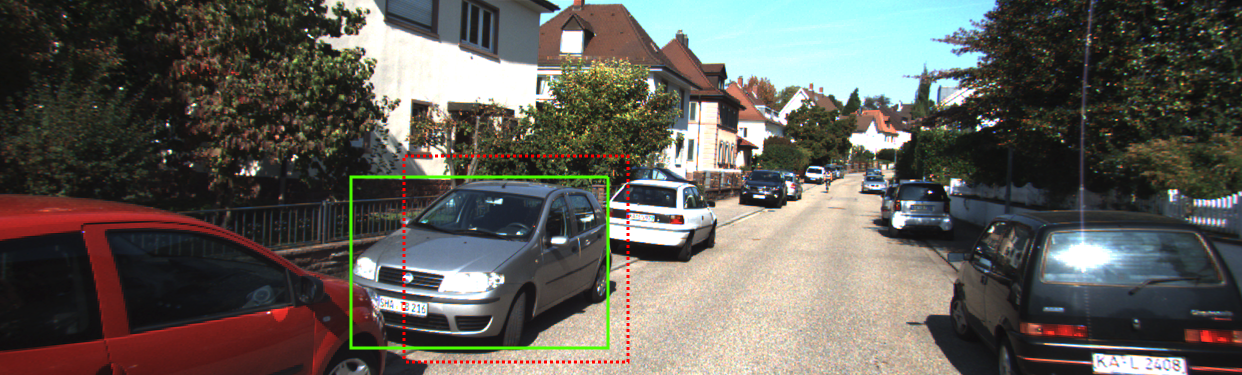
\includegraphics[width=1\textwidth]{../media/iou_img.png}
    \caption{Example of ground truth bounding box (solid green) and prediction bounding box (dashed red). In this image, the overlap between the green and red regions is the intersection, while the combined area is the union. The IOU of the two boxes is 0.64. Image index: 8.}
    \label{iou_img} %label goes last
\end{figure}

In order to formally calculate IOU, a generalized form may be generated to apply to n-dimensions. The generalized mathematical equation is simply as follows. Given a region A and a region B: 
\begin{equation}
IOU = \frac{|A\cap B|}{|A\cup B|} = \frac{|A\cap B|}{|A|+|B|- |A\cap B|}
\end{equation}

To assist in understanding IOU, a code snippet as well as an example are presented.

All aspects of calculating the IOU (including area and intersection) are broken up into multiple pieces, but presented together below. For n-dimensions, the code (presented here in python) is as follows: 


\begin{figure}[H]
\setstretch{0.84} % want code to be nice and compact
\begin{lstlisting}
import numpy as np

def extent(box,inclusive=False):
    '''
    Return the size or "extent" (length, area, volume, etc) of a given box in
        n-dimensions.
    INPUTS:
        box: n-dimensional bounds, format [x1,y1,z1, .. ,x2,y2,z2, ..]
        inclusive: boolean. add 1 unit to calculation, such as for image area
    OUTPUT:
        extent: size of box bounds, scalar float.
    NOTE:
    Internal convention: [Nx2] array,
        | x1 x2 |
        | y1 y2 |
        | z1 z2 |
        | .. .. |
    '''
    o= 1 if(inclusive) else 0 # add '1' if inclusive is true
    b=np.array(box).reshape((2,-1)).T # now in internal convention
    return np.product([i[1]-i[0]+o for i in b])
def intersection(box1,box2,inclusive=False):
    '''
    Return the size / "extent" of intersection between two bounds of
        n-dimension. Internal convention follows same as "extent" function.
    INPUTS:
        box1,box2: n-dimensional bounds, format [x1,y1,z1, .. ,x2,y2,z2, ..]
    OUTPUT:
        intersection: size of overlapping bounds, scalar float.
    '''
    o= 1 if(inclusive) else 0 # add '1' if inclusive is true
    b1=np.array(box1).reshape((2,-1)).T
    b2=np.array(box2).reshape((2,-1)).T # internal convention
    c=np.stack((b1,b2),2)
    # for each dimension, get (min(upperbound)-max(lowerbound)) and get product
    val=1
    for i in range(len(b1)):
        ans=np.min(c[i,1,:])-np.max(c[i,0,:])
        val*=max(ans,0) # if have negative dimension, have no intersection
    return val

def IOU(b1,b2,inclusive=False,criterion=-1):
    '''
    Return generalized intersection over union for two bounding boxes of
        matching n-dimension.
    INPUTS:
        b1,b2: n-dimensional bounding boxes, format [x1,y1,z1, .. ,x2,y2,z2, ..]
        inclusive: boolean, whether to include +1 unit, such as for images. default=False
        criterion: -1=div by union. 0 = div by extent(b1). 1 = div by extent(b2). default=-1
    OUTPUT:
        iou: intersection over union, scalar float, range [0,1].
    '''
    inter = intersection(b1,b2,inclusive)
    union = extent(b1,inclusive)+extent(b2,inclusive)-inter
    if(criterion==-1):
        return inter / union
    elif(criterion==0):
        return inter / extent(b1,inclusive)
    else:
        return inter / extent(b2,inclusive)

\end{lstlisting}
\onehalfspacing % set line spacing back to normal
\caption{Python implementation of generalized IOU calculation.}
\label{code_iou}
\end{figure}

\subsubsection{Example: IOU of a Ground Truth and Prediction Label}
Suppose there is an image, as given below, where there is a ground truth label `gt' and a prediction label `pred' with 2D bounding boxes formatted as \texttt{[x1,y1,x2,y2]}, all units in pixels. To determine the IOU of the image, the calculations are listed below. Because boxes represent pixel values, remember to add "1" to each dimension.



\def \pxpx {\ [px^2]}
\def \Asub #1{A\textsubscript{#1}}
\begin{enumerate}\itemsep=-0.5em
    \item Find area of each bounding box: \\ $\Asub{gt} = (x2-x1+1)*(y2-y1+1) = 16,335 \pxpx $ , $ \Asub{pr} = 12905 \pxpx $
    \item Find overlapping area, e.g. intersection (see \ref{code_iou} for more info): $I = 11455 \pxpx $
    \item Calculate IOU: $\frac{I}{\Asub{gt} + \Asub{pr} - I} = 0.644 $
\end{enumerate}

\begin{figure}[h] % h = "approx here", {h,t,b}
    \centering
    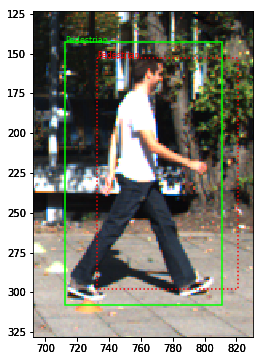
\includegraphics[width=.4\textwidth]{../media/iou_example.png}
    \caption{IOU calculation example. Ground truth (green solid) has BB: [712,143,810,307]. Prediction (red dotted) has BB: [732,153,820,297]. IOU is 0.644.}
    \label{iou_example} %label goes last
\end{figure}


\subsection{Precision \& Recall}
Once all detections have been tallied and placed into their correct categories, their precision and recall may be calculated. In information retrieval, precision is defined as "the fraction of retrieved documents that are relevant", and recall is defined as "the fraction of relevant documents that are retrieved". Reworded for object detection: precision is the number of correct predictions divided by the total number of predictions, and recall is the number of correct predictions divided by the total number of possible answers. These two are also given as equations in terms of true positives and so on. 

\begin{equation}
Precision = \frac{TruePositives}{TruePositives + FalsePositives}
\end{equation}

\begin{equation}
Recall = \frac{TruePositives}{TruePositives + FalseNegatives}
\end{equation}

In practice, the precision and recall of each detection is generated procedurally as each detection is compared to ...

KJG190618: NEED TO PERSONALLY RUN THROUGH A SIMPLE EXAMPLE OF PRECISION / RECALL, AND PUT THIS INTO YOUR PYTHON SANDBOX XX

% ABOUT THE KITTI DATASET ======================================================
\newpage
\section{About the KITTI Dataset}
\label{appendix_kitti}

\subsection{Introduction}
To better understand the actual data that is being worked on, the KITTI dataset will be explained in-depth here. KITTI itself is a combination of "KIT" (Karlsruhe Institute of Technology) and "TTI" (Toyota Technical Institute, Chicago), the two cooperating institutions on the project. The very first thing to know about the KITTI dataset is that it is actually a set of datasets, each dataset specialized for some specific AI task. This means that there are some number of evaluation tasks / benchmarks, and a not-necessarily-unique dataset is used to enable completion of that task. The individual tasks are listed below with a brief description: 

\begin{itemize}\itemsep=-0.5em 
    \item Stereo, Optical Flow, Sceneflow (2012 \& 2015): An older (2012) and updated (2015) task comprised of 200 training and 200 test scenes. Each scene consists of a left and right image as well as a "multi-view extension".
    \item Depth Completion / Estimation: A task comprised of about 93 thousand scenes containing RGB images and lidar scans.
    \item Visual Odometry / SLAM: 11 training and 11 testing stereo sequences with relevant grayscale, color, lidar, and ground truth poses.
    \item 2D / 3D / Bird's Eye View (BEV) Detection: 7481 training and 7518 test scenes with relevant color images, temporally preceding images, and lidar
    \item Single-/Multi- Object Tracking: An older (single) and in-development (multi) task consisting of multiple training and test sequences with relevant image, lidar, and GPS/IMU data. 
    \item Road / Lane Detection: Around 289 training and 290 test images used for detecting various road scenes, containing image and lidar information.
    \item Semantic / Instance Segmentation: A task comprised of a set of stereo images like the Stereo task, but containing pixel-level localization of each class. 
\end{itemize}

Each evaluation task also brings with it a "dev kit" (a set of files that explain some of the technical information as well as helpful code), relevant camera / sensor calibration data of some kind, as well as some kind of ground truth label / file for each scene to assist with training. It should be noted that raw data of each dataset is available as well, but these are often unused and only kept as original source files for transparency. Below in Figure \ref{kitti_samples} is an image summary taken from the various tasks to give a quick and simple overview of the variety of datasets.

\begin{figure}[H]
    \centering
    \subfigure[Stereo, Optical Flow, Sceneflow (2015)]{
        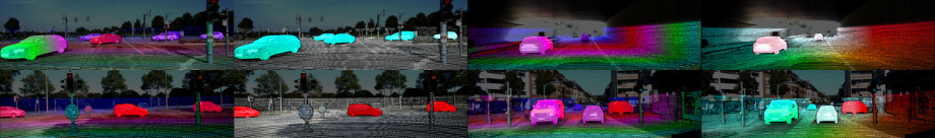
\includegraphics[width=1\linewidth]{../media/kitti_1_stereo.png}}
    \subfigure[Depth Completion, Depth Evaluation (2017)]{
        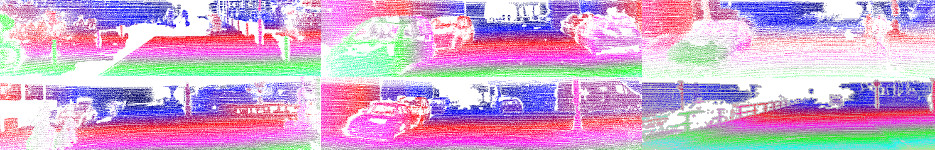
\includegraphics[width=1\linewidth]{../media/kitti_2_depth.png}}
    \subfigure[Visual Odometry / SLAM (2012)]{
        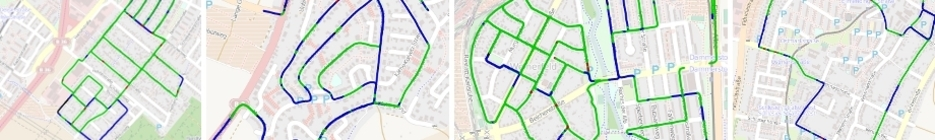
\includegraphics[width=1\linewidth]{../media/kitti_3_odom.png}}
    \subfigure[2D (2012), 3D (2017), Bird's Eye View (2017) Object Detection]{
        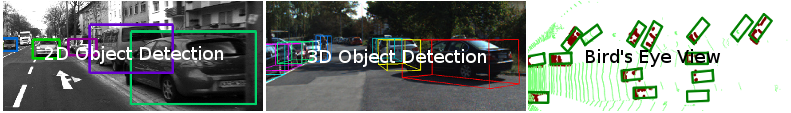
\includegraphics[width=1\linewidth]{../media/kitti_4_objdet.png}}
    \subfigure[Single Object(2012), Multi-Object (ongoing) Tracking]{
        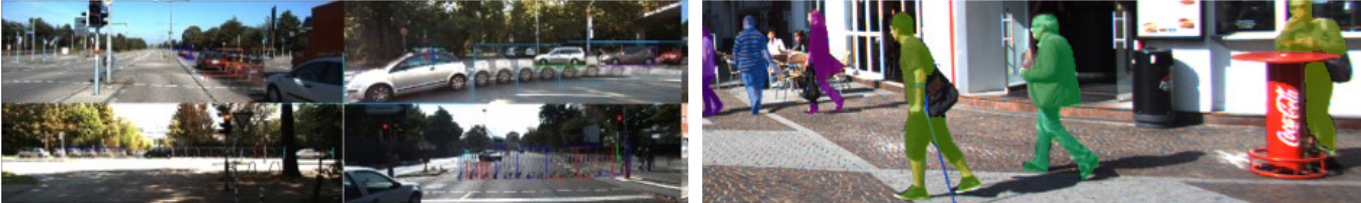
\includegraphics[width=1\linewidth]{../media/kitti_5_track.png}}
    \subfigure[Road / Lane Detection (2013)]{
        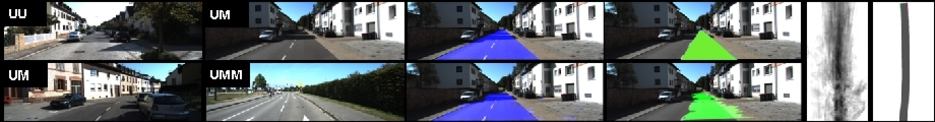
\includegraphics[width=1\linewidth]{../media/kitti_6_road.png}}
    \subfigure[Semantic and Instance Segmentation (2015)]{
        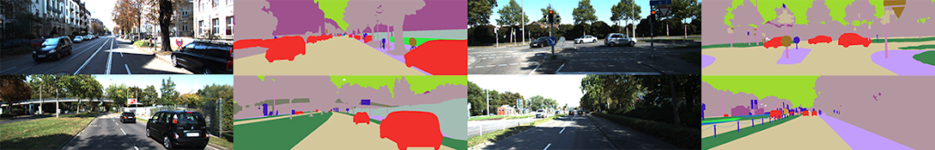
\includegraphics[width=1\linewidth]{../media/kitti_7_seg.png}}
    \caption{xx add more detail}
    \label{kitti_samples}
\end{figure}

Each task is associated with one or more papers published by KIT and TTI, but these will not all be listed here. Instead, we shall now explain two datasets, especially the most relevant one: the KITTI object detection dataset, referred to as the KITTI dataset.

\subsection{The Stereo Dataset}
The stereo dataset, specifically 2015, will be briefly covered to describe its merits as well as why it presented overlap issues with the object detection dataset. What makes the stereo dataset important is that it is the dataset that was initially used to finetune the Pyramid Stereo Matching network and also the dataset used to help it achieve such a high position in the stereo benchmark. 

The dataset itself is made up primarily of 200 training scenes and 200 testing scenes. The training scenes contain ground truth disparity maps, while the testing scenes do not and are used for final evaluation and submission to the benchmark website. For the project, only the training scenes were used. Each training scene is comprised of a left-hand side (LHS) color image, a RHS color image, a calibration file (containing transformation and other matrices), and a ground truth disparity file. There is also an available "multi-view extension", containing 20 extra frames per scene, but this was not used. Figure \ref{stereo_sample} below shows all relevant data in a single sample scene: the left and right images, as well as a disparity map ground truth.

\begin{figure}[H]
    \centering
    \subfigure[LHS image]{
        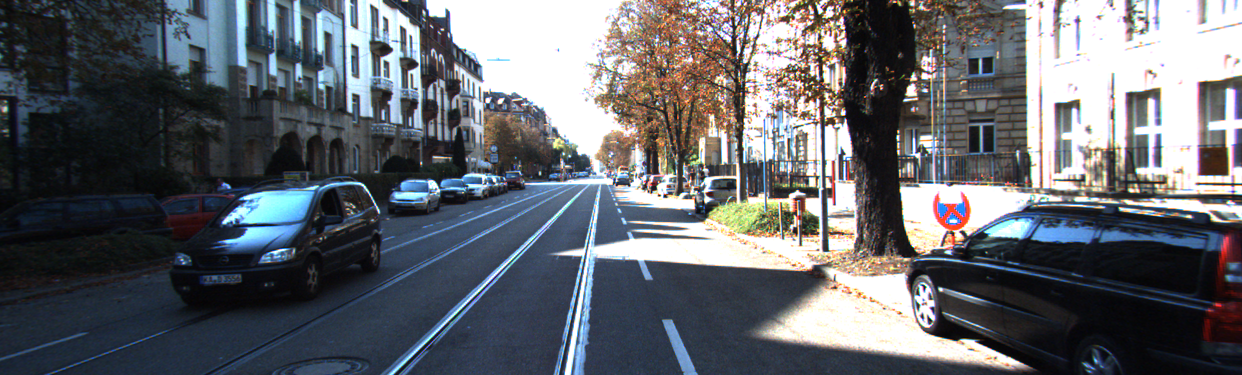
\includegraphics[width=0.487\linewidth]{../media/stereo_LHS_000000_10.png}}
    \subfigure[RHS image]{
        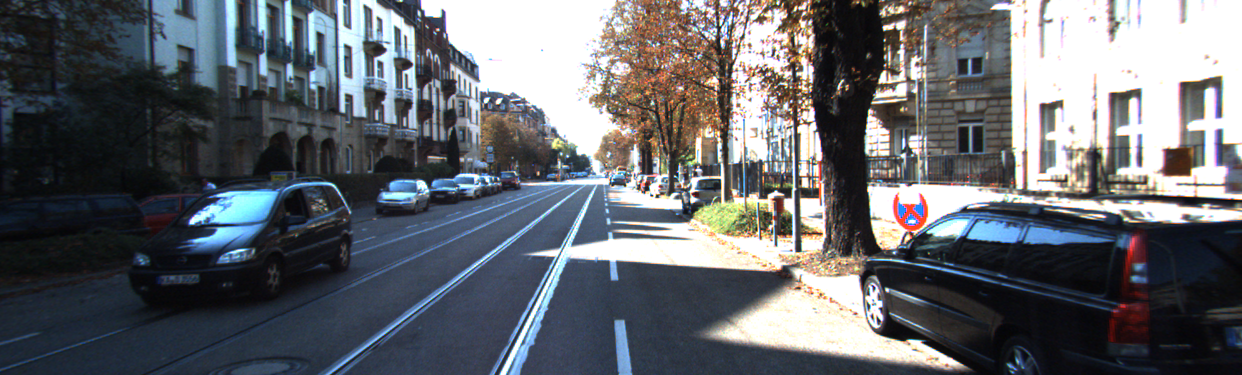
\includegraphics[width=0.487\linewidth]{../media/stereo_RHS_000000_10.png}}
    \subfigure[Ground truth disparity map with a viridis colormap. The value range for the original ground truth file may lie anywhere from 1 to 33,000 or a little higher. Disparity is a measure of how far apart one pixel is relative to its matching pixel in another location. ]{
        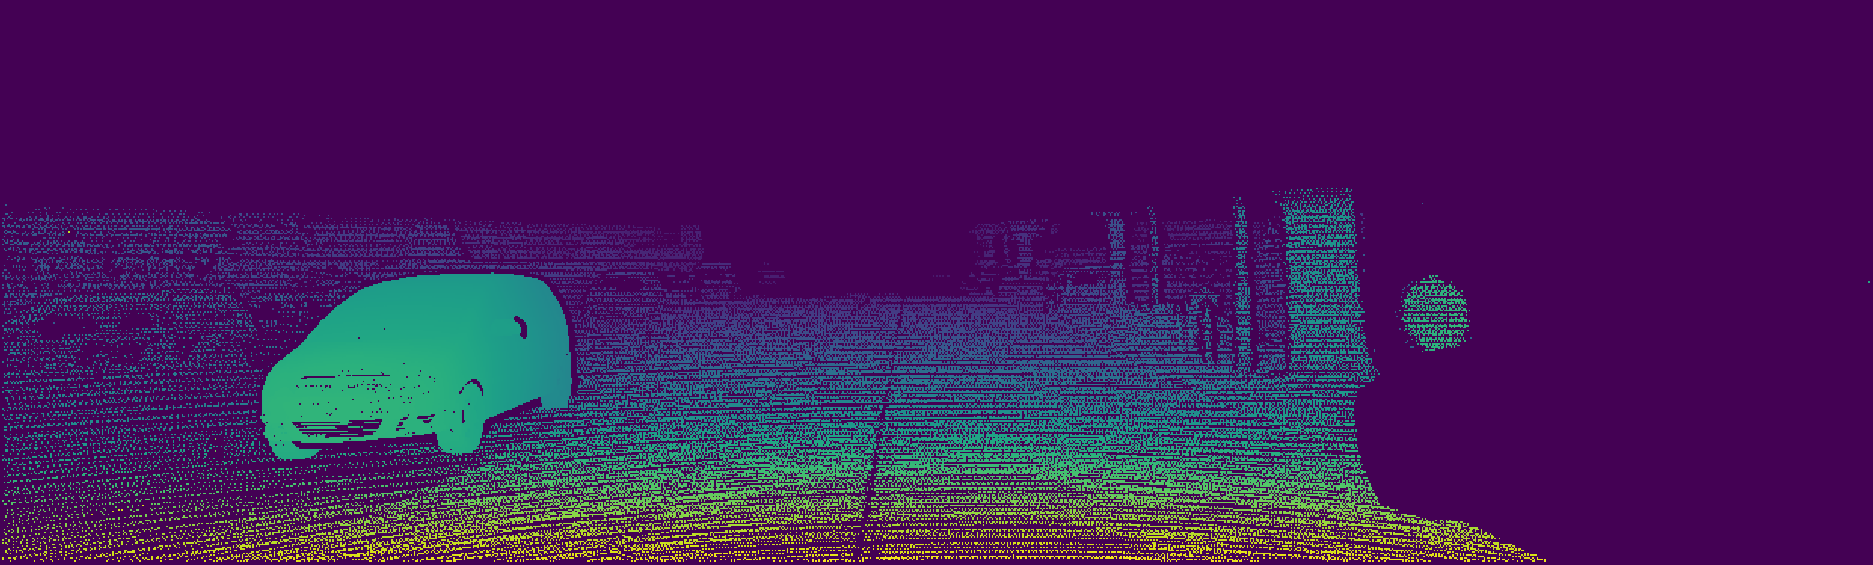
\includegraphics[width=1\linewidth]{../media/stereo_GTdisp_000000_10.png}}
    \caption{Sample scene from stereo dataset. Index 000000\_10}
    \label{stereo_sample}
\end{figure}

The ground truth labels were generated by a "semi-automatic" process, as described by Menze and Geiger: the process was to "extract disparity maps directly from the 3D information int he laser scans and fit geometrically accurate CAD models to moving 3D point clouds" \cite{Menze_2015_CVPR}. This explains several things about the ground truth disparity map in Figure \ref{stereo_sample}(c): the image is generally sparse, has no sample values above a certain horizontal line, and has a high density of pixels in the region where a car is outlined.

Ultimately, however, this dataset was not used for the primary reason described by \cite{wang_pseudo-lidar_2019}: there was an unacceptable amount of overlap, also known as data leakage, between the stereo dataset training data and the similar but unrelated object detection dataset. Figure \ref{similarity_stereo_objdet}, shown in Section 3, gives an example of a scene in the stereo dataset nearly matches a scene in the object detection dataset.

\subsection{The Object Detection Dataset \& Statistics}
The Object Detection dataset is the primary source of sensor data and media for this project, including PSMnet once it was determined that the stereo dataset had too much similarity with this dataset. The Object Detection dataset is comprised of 7481 training scenes and 7518 testing scenes. The testing scenes were ignored for the purposes of this project, since they are unlabeled for KITTI benchmarking. Each scene in the training dataset contains a LHS (left-hand side) image, RHS image, lidar data, calibration data, and ground truth labels. An example of the images and lidar are given below in Figure \ref{objdet_sample}. 

\begin{figure}[H]
    \centering
    \subfigure[LHS image]{
        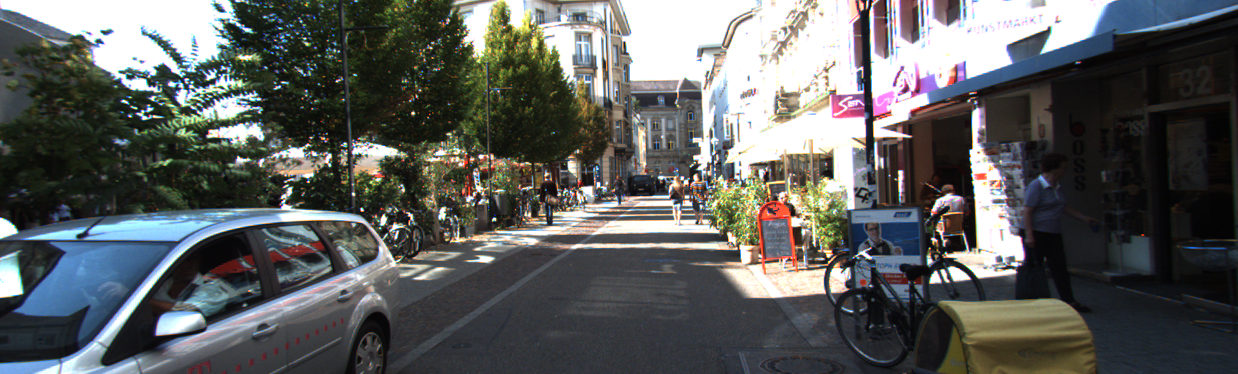
\includegraphics[width=0.487\linewidth]{../media/objdet_LHS_000015.png}}
    \subfigure[RHS image]{
        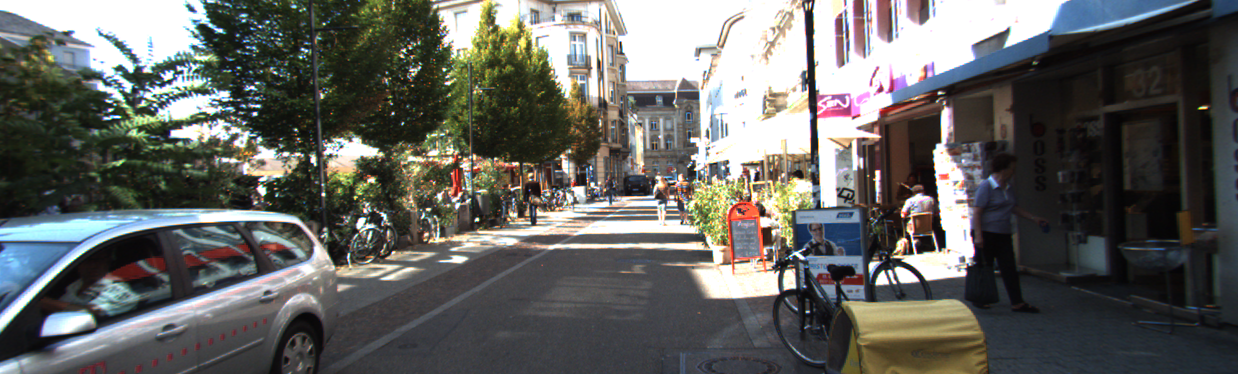
\includegraphics[width=0.487\linewidth]{../media/objdet_RHS_000015.png}}
    \subfigure[Velodyne lidar points projected onto image plane. Gray background for ease of viewing. Individual points use viridis colormap.]{
        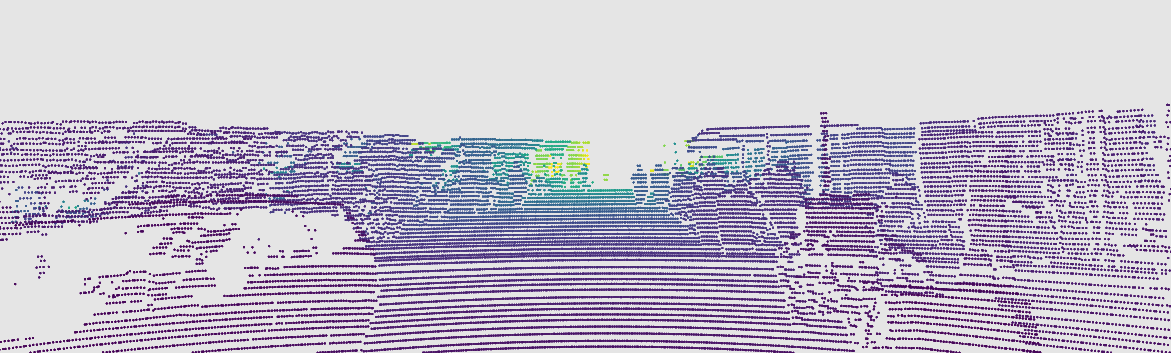
\includegraphics[width=1\linewidth]{../media/objdet_lidar_000015.png}}
    \caption{Sample scene from object detection dataset. Index 000015}
    \label{objdet_sample}
\end{figure}

In addition to the above lidar projection, the point cloud may be better visualized with an isometric view, rather than one from the camera's perspective. This is provided below, with white 3D bounding boxes provided for reference.

\begin{figure}[H]
    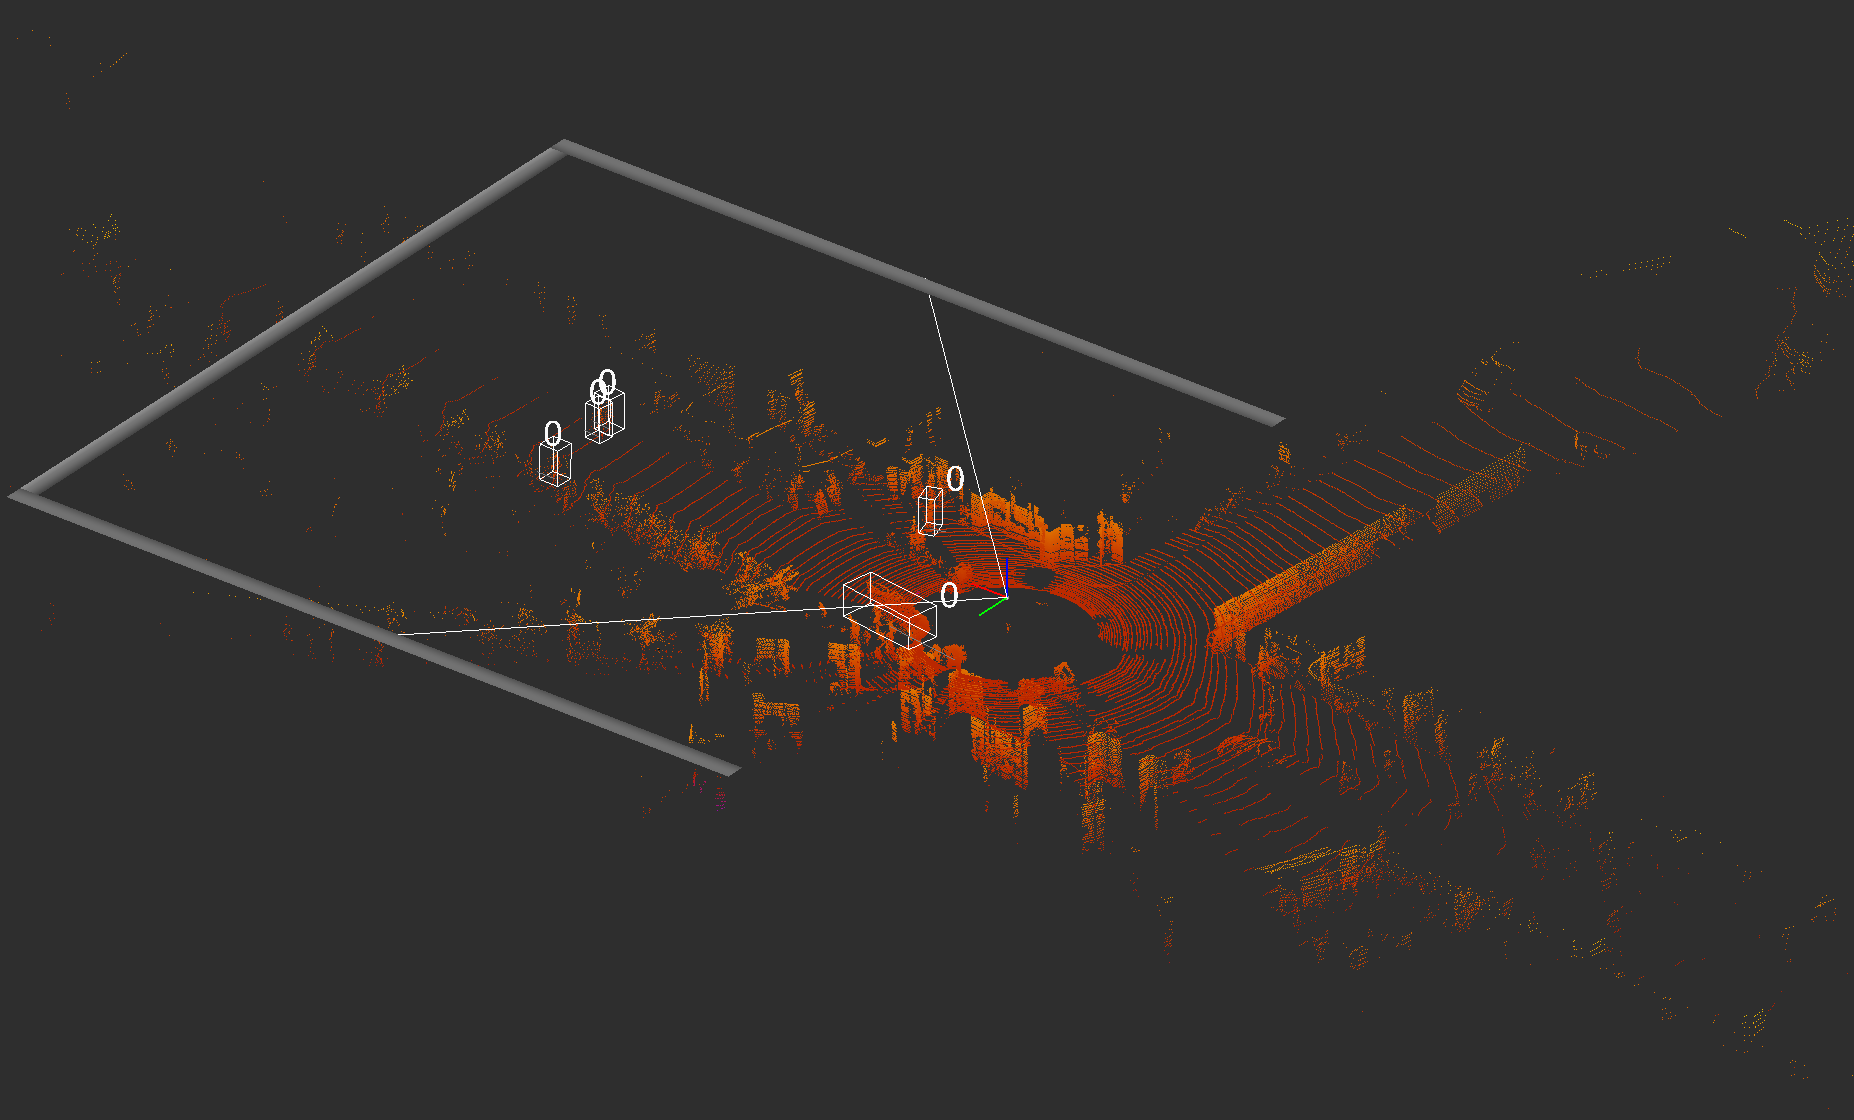
\includegraphics[width=1\linewidth]{../media/objdet_lidar_BEV_000015.png}
    \caption{Lidar pointcloud, alternate view. 3D bounding boxes are included as well as the horizontal field of view (white angled lines leading away from coordinate system origin). Index 000015}
    \label{objdet_lidar_sample}
\end{figure}

\def \DEG{$^{\circ}$} % Don't want to import extra package for no reason right now.

As is immediately obvious above in Figure \ref{objdet_lidar_sample} and from knowledge of the hardware itself, a lidar scan is capable of capturing points surrounding the sensor in a 360\DEG horizontal view. However, because of the nature of a typical color camera, points that are outside the camera's field of view are filtered out. 

Another key piece of the object detection dataset are the label data. Ground truth labels are simply lines of text that contain an array of information about each instance of an object in the scene. An example label with value names is given below in Table \ref{kitti_label_sample}. There are 15 values in each label, and an extra 16th "Score" value for prediction labels, a decimal in range [0,1]. The raw text for this label simply looks like so: \\
\texttt{Car 0.89 0 2.29 0.00 194.70 414.71 373.00 1.57 1.67 4.14 -2.75 1.70 4.10 1.72} \\


\begin{table}[h]
\centering
\caption{KITTI object detection sample label from a given scene. Index 000015}
\begin{tabular}{|c|c|c|c|c|c|c|}
\hline
Class & Trun & Occl & Obs  & BBx1  & BBy1   & BBx2  \\
\hline
Car   & 0.89       & 0         & 2.29 & 0.00  & 194.70 & 414.71 \\
\hline
\end{tabular}
\begin{tabular}{|c|c|c|c|c|c|c|c|}
\hline
BBy2   & HT   & WD   & DP   & Xc    & Yc   & Zc   & Roty \\
\hline
373.00 & 1.57 & 1.67 & 4.14 & -2.75 & 1.70 & 4.10 & 1.72 \\
\hline
\end{tabular}
\label{kitti_label_sample}
\end{table}

In order to better understand the meaning of each value, each dataset provides a "development kit" that contains a "readme.txt" file. In the object detection devkit, the following text reproduced in Figure \ref{kitti_devkit_info}. Some of the names are different than what is used, but the order and purpose are identical. 

\begin{figure}[h] %h=here,t=top,b=bottom,H=exactlyHere
	\setstretch{0.84} % want code to be nice and compact
	% note: optional line numbers argument
	\begin{lstlisting}[language=tex]
Ct.  Name         Description
----------------------------------------------------------------------------
1    type         Describes the type of object: `Car', `Van', `Truck',
                      `Pedestrian', `Person_sitting', `Cyclist', `Tram',
                      `Misc' or `DontCare'
1    truncated    Float from 0 (non-truncated) to 1 (truncated), where
                      truncated refers to the object leaving image boundaries
1    occluded     Integer (0,1,2,3) indicating occlusion state:
                      0 = fully visible, 1 = partly occluded
                      2 = largely occluded, 3 = unknown
1    alpha        Observation angle of object, ranging [-pi..pi]
4    bbox         2D bounding box of object in the image (0-based index):
                      contains left, top, right, bottom pixel coordinates
3    dimensions   3D object dimensions: height, width, length (in meters)
3    location     3D object location x,y,z in camera coordinates (in meters)
1    rotation_y   Rotation ry around Y-axis in camera coordinates [-pi..pi]
1    score        Only for results: Float, indicating confidence in
                      detection, needed for p/r curves, higher is better.
	\end{lstlisting}
	\onehalfspacing % set line spacing back to normal
	\caption{Original text from readme.txt file of devkit\_object resources. The columns are: Ct. ("count"), Name (of value), and Description.}
	\label{kitti_devkit_info} % label goes last
\end{figure}

Beyond a few samples of the dataset, some statistics about the dataset can be found in both the accompanying paper as well as by looking through the dataset itself. When observing only the training data, the count of each class can be described. A quick summary of each value across all labels in the training dataset is given below in Table \ref{kitti_label_stats}. Note that the min/max range ignores the DontCare class and its values, such as -1000 for $z_c$.

\begin{table}[h]
	\centering
	\caption{KITTI dataset label statistics. Each numbered value's minimum and max values are given. Xc, yc, and zc are distance to the bounding box center of mass, and pixel values are given to sub-pixel accuracy.}
	\begin{tabular}{|c|c|c|c|c|}%
		\hline
		\bfseries Name & \bfseries DataType & \bfseries Unit & \bfseries min & \bfseries max % specify table head
		\csvreader[head to column names]{../media/kitti_label_stats.csv}{}% use head of csv as column names
		{\\\hline\csvcoli&\csvcolii&\csvcoliii&\csvcoliv&\csvcolv} % specify your columns here
		\\\hline
	\end{tabular}
	\label{kitti_label_stats}
\end{table}

The final bit of interesting statistical information may be found by counting the number of instances of each class. This is already provided by \cite{geiger_are_2012}, but in verifying the values provided only in the training data the exact number of instances of each class are listed below in Table \ref{kitti_class_stats}. 

\begin{table}[h]
	\centering
	\caption{KITTI object detection class count. Semi-automatically counted through only labeled training data.}
	\begin{tabular}{|c|c|}
		\hline
		\bfseries Class & \bfseries Count\\
		\hline
		Car & 28742 \\
		\hline
		Pedestrian & 4487 \\
		\hline
		Van & 2914 \\
		\hline
		Cyclist & 1627 \\
		\hline
		Truck & 1094 \\
		\hline
		Misc & 973 \\
		\hline
		Tram & 511 \\
		\hline
		Person\_sitting & 222 \\
		\hline
	\end{tabular}
	\label{kitti_class_stats}
\end{table}

\subsection{Evaluation Difficulty Levels}
One of the last but certainly not least important aspects of the KITTI dataset is the multi-level difficulty rating system. The KITTI dataset certainly has a variety of scenes and training data, but it also allows scoring to be performed on three difficulty levels, defined as follow: 

\begin{enumerate}\itemsep=-0.5em
	\item Easy: Min. bounding box height: 40 Px, Max. occlusion level: Fully visible, Max. truncation: 15\%
	\item Moderate: Min. bounding box height: 25 Px, Max. occlusion level: Partly occluded, Max. truncation: 30\%
	\item Hard: Min. bounding box height: 25 Px, Max. occlusion level: Difficult to see, Max. truncation: 50\%
\end{enumerate}

Naturally, the "Easy" difficulty typically earns a higher AP score than "Moderate", and "Moderate" in turn typically yields a higher AP score than "Hard". The official final score that a network receives when submitted to the KITTI Leaderboard is the "Moderate" mean AP score. This paper specifically deals with the "Car" class, so we may be able to better understand how these difficulties affect other parameters. Specifically related to the "Car" class, 3D bounding box is considered a detection at 70\% overlap with a ground truth. The other two classes, "Pedestrian" and "Cyclist", only require an overlap of 50\%. The remaining other classes are not typically included in evaluation and scoring. 

In the paper \cite{wang_pseudo-lidar_2019}, the "Easy" evaluation for the "Car" class is said to test on car labels located mostly within 30m of the ego vehicle, which was also claimed by another group, [CITE NEEDED XX]. This was verified, and it is described below in Figure \ref{kitti_labels_easyCar}. 

\begin{figure}[h] % h = "approx here", {h,t,b}
	\centering
	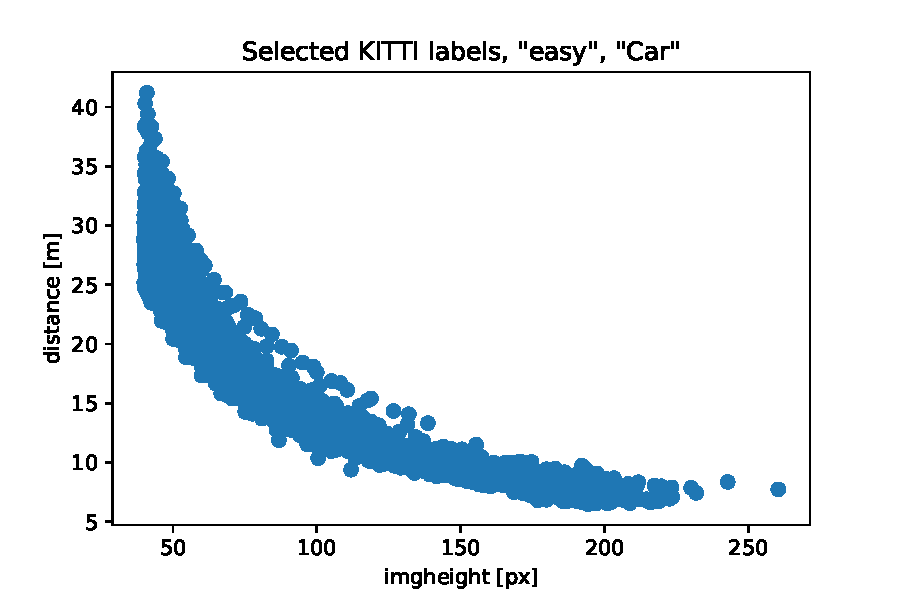
\includegraphics[width=0.5\textwidth]{../media/kitti_labels_easyCar.pdf}
	\caption{Filtered set of labeled training data containing only labels with the "Car" class and those which are defined as "Easy" difficulty. Specifically, there are 199 labels with a distance farther than 30m, while there are a total of 5971 filtered labels, meaning just over 3\% of these filtered labels are beyond 30m, verifying the claim of other papers. An interesting observation that may be made from the pixel height / distance relationship is that they are inversely correlated.}
	\label{kitti_labels_easyCar} %label goes last
\end{figure}


% 3D RECONSTRUCTION ============================================================
\newpage
\section{3D Reconstruction from Stereo Data}
\label{appendix_reconstruct}
Reconstruction is the process of taking a series of 2D images and producing a 3D representation of that information (CITATION NEEDED XX). In this project, reconstruction is a vital part of taking the disparity map estimation of one network and creating a pointcloud that is given to the second network. This appendix will provide a more hands-on description of converting from a disparity map to a pointcloud. 

A disparity map consists of a 2D matrix that may be considered analog to a normal grayscale image, but the value at each (row,column) location represents disparity, or the horizontal (normally) distance between two matching pixels in two different images. Using some basic equations, disparity may be manually calculated. Let there be two cameras, able to produce left and right color images where a ball can be seen, and are able to produce rectified images (images that have corrected the barrel / pincushion distortion). If the cameras are spaced a known distance apart, then their respective images will each contain the ball at some horizontal pixel distance from the left edge of each image. If the ball is located at 100 pixels away from the edge in the left image and 150 pixels away in the RHS image, then the disparity is 50 pixels. Thus, a disparity map may be generated by looking for matching features in two images and assigning each location a difference in the value of where one is found in reference to another (typically the LHS image is the reference).

The reason for this explanation is that a disparity map must then be transformed into a pointcloud by relating the disparity value at each pixel to a depth distance and the row / column locations to vertical / horizontal distances, respectively. This is accomplished through epipolar formulas, as mentioned in \ref{sect_reconstruct}, which are as follow: 

\begin{equation}
z = \frac{f_U * b}{D}
\end{equation}

\begin{equation}
x = \frac{(u - c_U) * z}{f_U}
\end{equation}

\begin{equation}
y = \frac{(v - c_V) * z}{f_V}
\end{equation}

In these equations, $D$ stands for a disparity matrix, $f_U$ and $f_V$ are for horizontal \& vertical focal lengths (respectively), ($c_U$,$c_V$) are the pixel center of the image, and $(u,v)$ represent a (column, row) coordinate location in $D$.

KJGNOTE NEED TO CONTINUE THIS SECTION XX



% LIDAR COST EFFECTIVENESS =====================================================
\newpage
\section{Lidar vs Other Sensors: Economic Perspective}
\label{appendix_lidar}
TextNeededHere


Alright, would like to deal with a way of comparing lidar vs other sensors in the economic sense, but need some standards to actually perform a comparison. for one, how about we start with what a single frame. in a single frame, we may ask ourselves... how much information do we really have? if for example, a lidar sensor can give you 100 pts in a horizontal 360 deg and vertical 1 deg field of view, what is the ... points per area that you're getting? 


the next thing you want to have is some kind of measure of quality. so, in order to measure quality, perhaps you want to know how much error you have. perhaps you would want to know the error at a given distance. so here, why not have a... centimeters per meter measure? 

finally, in order to deal with all these things on money terms, perhaps also consider... points per dollar. ideally, you want a dense, high quality image that isn't too expensive. saying that you get x amount of data per dollar perhaps also informs someone how effectively their money is being spent. 

let's take two examples from the lidar industry and give them some info. 

first up is the HDL-64E, which was used for the KITTI dataset. 

first, the base stats will be given: 


HDL-64E:
range: 120 m
pts/s: 1,000,000/s (10Hz)
cost: \$85,000 (2017)

%https://www.velodynelidar.com/lidar/products/manual/HDL-64E%20Manual.pdf
%https://medium.com/self-driving-cars/velodyne-lidar-price-reduction-d358f245f086
%https://driverless.wonderhowto.com/news/quanergys-new-250-solid-state-lidar-could-bring-self-driving-masses-0175790/













kjg190617: quick note on area of sphere
$$ A_{sphere}=R^2\theta \int_{a}^{b}\cos\phi*d\phi $$

$$ A_{sphere}=R^2\theta (\sin{b} - \sin{a})$$



% SAMPLE =======================================================================
\newpage
\section{Sample Appendix}
TextHere

\begin{figure}[h] % h = "approx here", {h,t,b}
    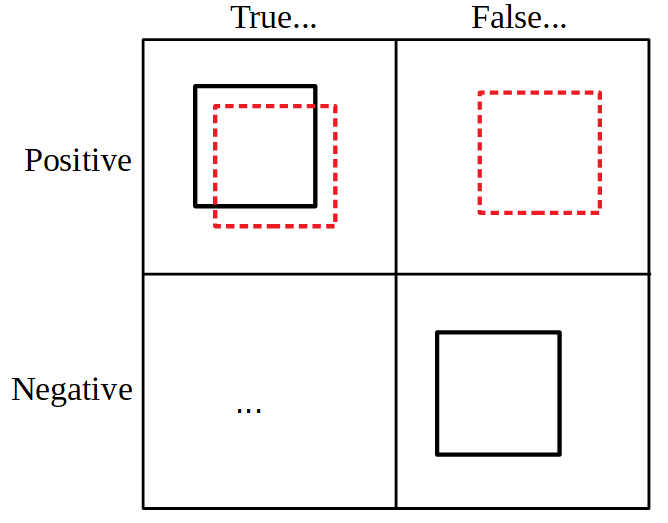
\includegraphics[width=1\textwidth]{../media/tp_help.png}
    \caption{texthere}
    \label{delme_figure} %label goes last
\end{figure}


\begin{figure}[h] %h=here,t=top,b=bottom,H=exactlyHere
\setstretch{0.84} % want code to be nice and compact
% note: optional line numbers argument
\begin{lstlisting}[numbers=left]  %note: 'tex' is for 
def pyt(a,b):
    return (a**2+b**2)**0.5
\end{lstlisting}
\onehalfspacing % set line spacing back to normal
\caption{Python implementation of generalized IOU calculation.}
\label{delme_code} % label goes last
\end{figure}

\begin{table}[h]
\centering
\caption{KITTI object detection sample label from a given scene. Index 000015}
\begin{tabular}{|c|c|c|c|c|c|c|}
\hline
Class & Trun & Occl & Obs  & BBx1  & BBy1   & BBx2  \\
\hline
Car   & 0.89       & 0         & 2.29 & 0.00  & 194.70 & 414.71 \\
\hline
\end{tabular}


\label{SampleTable}
\end{table}


%\begin{enumerate}\itemsep=-0.5em
%	\item one
%	\item two
%	\item three
%\end{enumerate}
